\section{El concepto de movimiento}

\begin{floatingfigure}[r]{8cm}
  \centering
  \href{https://commons.wikimedia.org/wiki/File:Leaving_Yongsan_Station.jpg#/media/File:Leaving_Yongsan_Station.jpg}{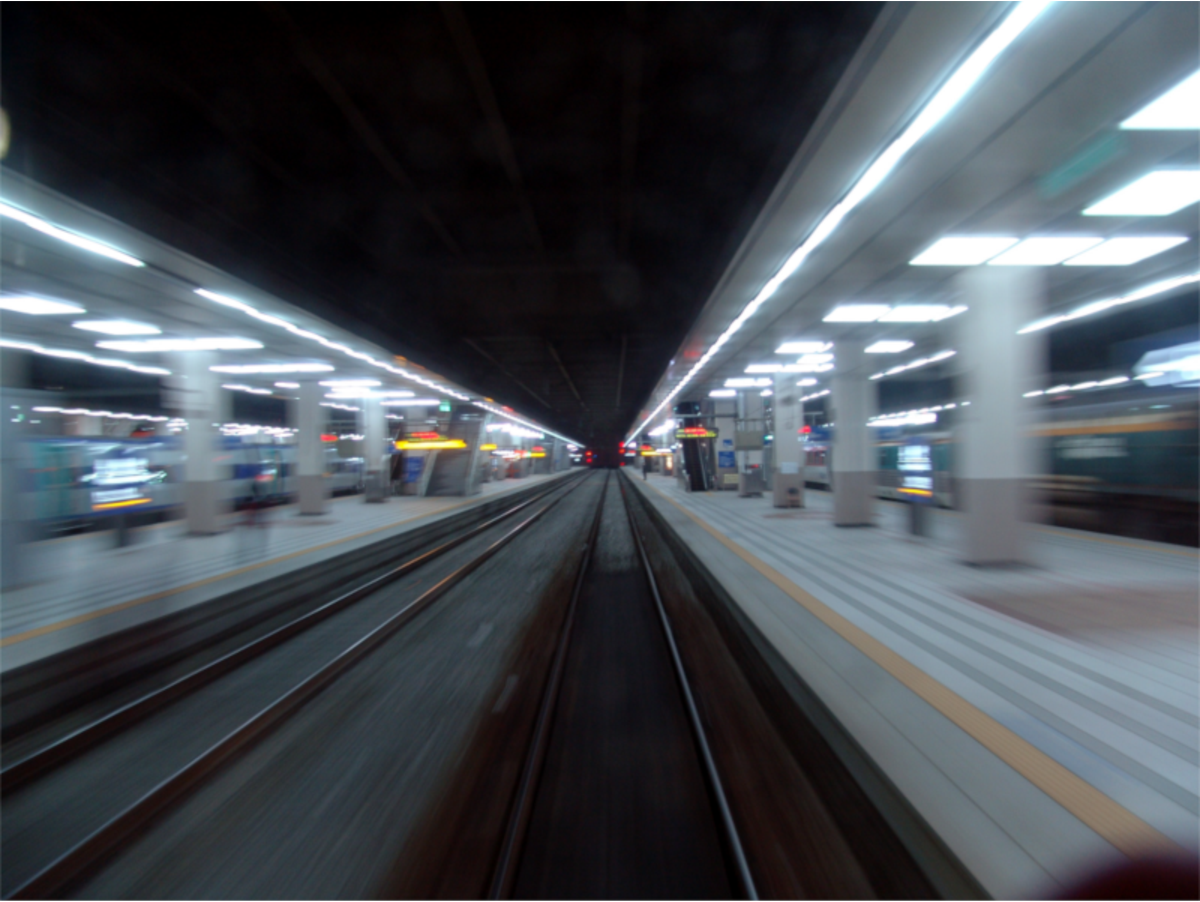
\includegraphics[width=7.5cm]{img/yongsan.pdf}}
  \caption{La estación Yongsan, en Seúl (Corea del Sur), fotografiada desde un tren. ¿Se mueve el tren o se mueve la estación? (Fuente: Wikimedia Commons - CC--BY-SA 3.0)}
\end{floatingfigure}

{\small{
  {\it Dos amigos viajan en el rápido de Buenos Aires a Rosario. Uno de ellos dice:}
  
  --¿En qué estará pensando ese señor que desde que salimos de Buenos Aires mira por la ventanilla y no se ha movido para nada?
  
  {\it El otro es un físico. Siente gusto por la discusión, por las definiciones precisas y un poco también por las bromas. Le responde:}
  
  --¿Cómo que no se ha movido? ¡Lleva recorridos unos 30 kilómetros a razón de 100 kilómetros por hora!
  
  --¡Vamos! Quiero decir que {\bf él} no se ha movido, que desde que empezó el viaje ha estado clavado en su asiento, mirando por la ventanilla, sin moverse una sola vez para nada. ¿Está claro?
  
  --No te exaltes. Más bien deberías avergonzarte de emplear las palabras tan a la ligera.
  
  --No entiendo...
  
  --Esto de hablar de moverse o no moverse es cosa peligrosa; las palabras deben emplearse con sumo cuidado. En primer lugar, fíjate que la discusión empezó porque olvidaste decir algo muy, pero muy importante.
  
  --Te olvidaste de aclarar {\bf con respecto a qué}, oye bien, con respecto a qué ese señor no se había movido. Reflexiona, que ese detalle es de importancia decisiva. En efecto: el señor no se ha movido respecto del vagón, con relación al vagón, a su asiento, a la ventanilla, si quieres. Pero en cambio se ha movido ¡y de qué manera! con relación a la ciudad de Buenos Aires. Se ha movido por lo menos 30 kilómetros, o ya 34, porque esta discusión debe llevar ya unos 4 kilómetros, si mi reloj y mi ojo no me engañan.
  
  --¡Bah! Todo eso son sutilezas y afán de discutir porque sí. No me vas a decir que toda esa palabrería tiene importancia.
  
  --¡Cuidado! Muchos grandes descubrimientos de la Física fueron hechos gracias a análisis como este, que tú calificas de palabrería. ¡Si supieras lo que Galileo, Newton y Einstein aprovecharon de discusiones así...!
  
  --Bien, señor profesor, gracias por la lección. ¿Quiere decirme, entonces, de qué manera hay que expresarse para no suscitar las iras de físicos o ingenieros o astrónomos?
  
  --No tengo inconveniente alguno. Más todavía: estoy dispuesto a confesar que experimentaré un gran placer, pero con la condición de que respondas cada vez que te haga una pregunta. Te quiero probar que tú mismo eres capaz de sacar consecuencias interesantes.
  
  --A ver...

  --Primero, supongamos que estás en el andén de una estación, adonde has ido para despedir a tu familia. ¿Cómo sabes que el tren se pone en movimiento?
   
  --Pues, porque veo que las ruedas empiezan a moverse.
   
  --No hay necesidad de ver las ruedas. Eso es lo importante. Además, las ruedas podrían girar y patinar en el mismo lugar, de modo que el tren quedaría todavía en reposo.
   
  --Pues… simplemente porque se aleja.
   
  --Estamos de acuerdo, pero si agregas un detalle ¿Se aleja de quién? ¿Respecto de qué? ¿Con relación a qué?
   
  --Pues, porque se aleja de mí, con respecto a mí, con relación a mí.
   
  --Muy bien; progresas. Veamos si eres capaz, ahora, de decirme cuándo un cuerpo cualquiera está en movimiento.
   
  --Muy sencillo. Un cuerpo está en movimiento cuando aumenta su distancia respecto de un hombre que está en un lugar.
   
  --Bastante bien, pero con dos defectos.
   
  --¿Cuáles son?
   
  --Primer defecto: según tu definición, el tren se movería cuando se va, pero no cuando viene.
   
  --Me olvidé, claro. Habría que decir ``cuando {\bf aumenta} o {\bf disminuye} su distancia''.
   
  --Sí. Pero ahora viene el segundo defecto. Según tu definición, el tren sólo se mueve si hay un hombre parado en la estación. ¿Y si no hubiera nadie, el tren no se movería lo mismo?
   
  --Bueno, claro que no es necesario que haya un hombre allí.
   
  --Entonces, ¿cómo te parece que sería correcto decir?
   
  --Un cuerpo está en movimiento cuando aumenta o disminuye su distancia respecto de un punto fijo.
   
  --Muy bien, bastante bien para un aficionado. Fíjate, sin embargo, que el problema no queda todavía resuelto. Hay mucho que hablar.
   
  --¡Cómo! ¿Todavía?
   
  --Ya lo creo. Queda algo muy importante, de enorme importancia. ¿Quién se mueve, el tren o la estación?
   
  --¡Estás bromeando…!
   
  --Hablo en serio.
   
  --No sé adónde quieres ir a parar con esa pregunta de locos, pero te responderé como si fuera una pregunta cuerda. Es el tren el que se mueve.
   
  --Así que la estación está en reposo, ¿no?
   
  --Por supuesto.
   
  --¿Y no se te ha ocurrido pensar que la estación instalada en un planeta que se mueve vertiginosamente por los espacios siderales?

   {\it Aquí el amigo del físico se llevó la mano derecha al mentón, frunció el entrecejo, reflexionó, y finalmente dijo, casi con pavor:}
   
  --¡Caramba! Me parece que lo mejor en la vida sería no pronunciar ni una sola palabra. Creo que todo es terriblemente difícil. Me acabas de hacer ver algo increíble... En efecto… Claro... Entonces, si la estación está sobre la Tierra, y si la tierra gira y se traslada vertiginosamente en el espacio... Diablos... Es la misma cosa de hoy, con el señor ese y la ventanilla y la estación... Estamos como al comienzo... ¡Por el amor de Dios! ¿Me puedes decir qué es lo verdadero y qué es lo falso? ¿Quién se mueve? ¿Quién está en reposo? Ya no entiendo nada.
   
  --Ahora tienes verdadero interés; ahora no estás fastidiado por la palabrería, ¿no es así?
   
  --Lo confieso. Me muero de curiosidad.
   
  --Muy bien. Como decía un filósofo griego, el asombro es la madre de la sabiduría. Hay que empezar por asombrarse y preguntar, como los chicos: ¿por qué?, ¿por qué?
   
  --Bueno; responde de una buena vez.
   
  --Pues, en cierto modo, la respuesta es muy simple. Todos los movimientos son relativos, es decir, {\bf con relación a algo}, a un punto. Por ejemplo, para empezar con nuestro señor, el que originó la discusión, ese señor, está en reposo con relación al vagón, pero también podemos invertir la frase diciendo que el vagón está en reposo respecto al señor. Pero ese señor está en movimiento con respecto a la estación...
   
  --¿De modo que alguien o algo puede estar {\bf a la vez en reposo y en movimiento}?
   
  --Exacto. Todo depende del punto de referencia que se elija como fijo. Como decía, ese señor se mueve respecto a ese señor, considerándolo a él como fijo. No hay más derecho a decir lo primero que lo segundo, pues la estación no es ningún ente privilegiado, ya que pierde inmediatamente su jerarquía o su importancia en cuanto pensamos en el Sol o las estrellas. ¿Acaso la estación está en reposo respecto del Sol? De ningún modo.
   
  --¿Entonces?
   
  --Entonces, si queremos ser verídicos y no decir más que lo que debemos decir, habrá que definir el movimiento de esta manera...
   
  --Un momento, intentaré hacerlo yo.
   
  --Veamos...
   
  --Yo diría que ``un cuerpo está en movimiento con relación a un punto elegido como fijo, cuando aumenta o disminuye su distancia respecto a ese punto''.
   
  --¡Magnífico! Se puede todavía hacer una simplificación. En Física hay que emplear siempre el mínimo de palabras, y acá sobran dos.
   
  --A ver... ¡Ya sé!: {\bf ``Un cuerpo está en movimiento con relación a un punto elegido como fijo, cuando varía su distancia a ese punto''}.
   
  --Muy bien. Ahora tú mismo puedes extraer algunas conclusiones bastante curiosas sobre fenómenos que son bien conocidos. ¿Qué me podrías decir sobre dos trenes expresos que corren uno al lado del otro, en la misma dirección, el mismo sentido y con la misma velocidad?
   
  --Que un tren está en reposo con respecto al otro.
   
  --Perfecto. ¿Qué me podrías decir si uno de esos trenes se mueve a 100 kilómetros por hora y el otro a 90?
   
  --Que el primero se mueve a 10 kilómetros por hora con relación al segundo.
   
  --¡Magnífico! Creo que la lección ha sido provechosa. Puede sentarse, joven. Le pondré diez puntos.
   
  --¡Un momento, señor profesor! Me parece que la definición que usted acepta tiene un defecto.
   
  --¡Esto sí que está bueno! Así es, tiene un defecto. Si has dado en el clavo, resultarás mejor alumno de lo que yo esperaba. ¿Cuál es el defecto?
   
  --¿Qué pasa si revoleo una piedra y elijo como punto fijo mi hombro? La piedra recorre una circunferencia cuyo centro es mi hombro. La distancia de la piedra a mi hombro no varía, y sin embargo, la piedra se mueve.
   
  --Ese es el defecto. Para definir el movimiento con toda precisión, debe elegir no un punto de referencia, sino un {\bf sistema de referencia}. Pero, ¿recuerdas lo que es sistema de referencia?
   
  --Sí... tres rectas que se cortan en un mismo punto.
   
  --Y cada una perpendicular a las otras dos. Como las aristas de las paredes de una habitación que concurren a un mismo rincón. Y ahora, en lugar de decir: “Un cuerpo está en movimiento con relación a un punto cuando varía su distancia respecto de ese punto...”
   
  --Déjamelo decir a mí: ``Un cuerpo está en movimiento con relación a un sistema de referencia, elegido como fijo, cuando varían... ¡sus coordenadas en ese sistema!''
   
  --Bueno, hombre ahora tendría que ponerte diez y felicitarte...

  \bigskip
   \begin{flushright}
  {   \small{\it Texto adaptado del libro ``Física 1'' de Maiztegui y Sábato (2da ed. Kapeluz, 2005).}}
\end{flushright}
}}


\defin{Movimiento}

{\bf Un cuerpo está en movimiento con relación a un sistema de referencia elegido como fijo, cuando sus coordenadas en ese sistema varían a medida que transcurre el tiempo.}


\defin{Sistema de referencia}

Para describir un movimiento, un {\bf observador} elige un objeto o un conjunto de objetos que considera {\bf fijos} y allí coloca un conjunto de ejes de coordenadas. Este conjunto de ejes de coordenadas, {\bf en reposo con respecto al observador}, es lo que denominamos {\bf sistema de referencia}.

El concepto de movimiento se refiere a la modificación de la posición relativa de los cuerpos entre sí, por eso es necesario definir un sistema de referencia.
\begin{center}
  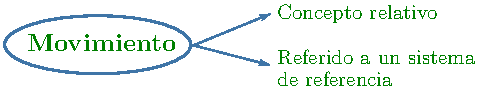
\includegraphics[scale=1.2]{img/movimiento.pdf}
\end{center}

El sistema de referencia tiene tanta importancia que no podemos hablar de reposo o de movimiento si no hablamos simultáneamente del sistema de referencia a partir del cual tenemos esa condición de reposo o de movimiento.

{\bf El sistema de referencia} es arbitrario y puede ser elegido por el observador de la forma que lo crea más conveniente para la descripción del movimiento que esté estudiando, {\bf pero una vez seleccionado debe ser mantenido invariable}.


\begin{figure}[H]
\centering
\begin{minipage}{.4\textwidth}
  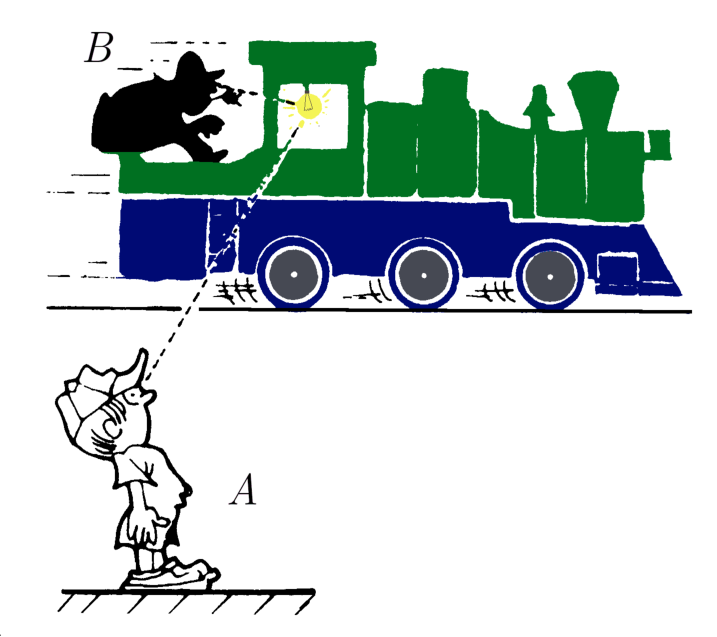
\includegraphics[width=\textwidth]{img/tren.pdf}
  \caption{La lámpara está inmóvil en relación con el observador $B$, pero se encuentra en movimiento en relación con el $A$.}
\end{minipage}%
\hfill
\begin{minipage}{.55\textwidth}
  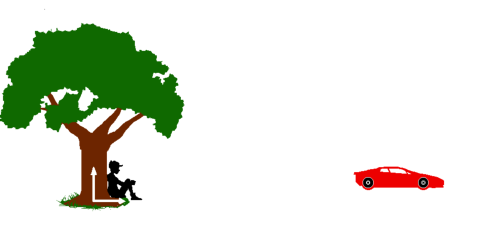
\includegraphics[width=\textwidth]{img/arbol.pdf}
  \caption{En la figura se ve un observador que ve alejarse un auto, ha elegido un sistema de  referencia (el árbol) y en él ha fijado un sistema de coordenadas, en este caso un sistema de ejes ortogonales.}
\end{minipage}
\end{figure}
    
\begin{comprension}
Retomando el ejemplo del tren: elige distintos sistemas de referencia y determina para cada uno qué cuerpos se mueven y qué cuerpos permanecen en reposo: persona parada en el andén de la estación, tren en marcha, persona sentada en el tren, persona caminando por el pasillo del ómnibus.
\end{comprension}


\defin{Partícula}

Un auto que se mueve por una autopista experimenta un movimiento de traslación, sus ruedas tienen un movimiento rototraslacional y además existe un movimiento vibratorio en todas sus partes.

En esta Unidad, abordaremos sólo el movimiento traslacional y específicamente el movimiento rectilíneo de partículas. Pero, ¿qué es una partícula?

Llamamos {\bf cuerpo puntual} o {\bf partícula} a todo cuerpo cuyas dimensiones son despreciables frente a las distancias que recorre. 

Por ejemplo, la Tierra puede ser considerada partícula en su movimiento orbital como planeta, puesto que la distancia Tierra--Sol es muchas veces mayor que el radio terrestre. En cambio, no puede ser considerada partícula cuando se estudian fenómenos como las mareas o los terremotos o cuando se examina su estructura interna.
En una escala mucho más pequeña, es posible explicar la presión ejercida por un gas sobre las paredes de un recipiente considerando las moléculas de gas como partículas, por otro lado no las podemos considerar partículas cuando se estudian propiedades que dependen de la rotación y vibración molecular. 

Vamos a trabajar, por ahora, con el {\bf \color{NavyBlue} modelo de partícula}. Con este modelo a los cuerpos los representamos por puntos.

\begin{comprension}
Piensa en un cuerpo cualquiera y menciona un ejemplo en el que se lo pueda considerar partícula y otro en el que no se pueda.
\end{comprension}

\defin{Trayectoria}

{\bf Conjunto de puntos del espacio que ocupa la partícula a lo largo de su movimiento.}

Un ejemplo de trayectoria es la ``línea dibujada'' por una abeja al volar por el jardín. Esta es una trayectoria muy complicada, como lo es también la trayectoria de una pelota durante un partido de fútbol.

Si la trayectoria es una curva, el movimiento es curvilíneo. Existen muchos movimientos curvilíneos diferentes, entre ellos podemos mencionar, en particular, los movimientos circulares y los parabólicos.

Si la trayectoria está contenida en una línea recta, {\bf el movimiento es  rectilíneo}.



\begin{figure}[!h]
\centering
\begin{minipage}{.55\textwidth}
  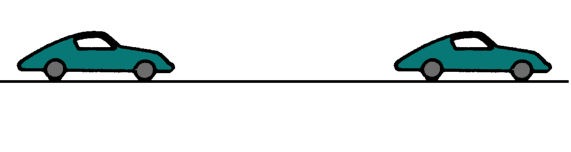
\includegraphics[width=\textwidth]{img/tray_rect.pdf}
  \caption{Una trayectoria rectilínea}
\end{minipage}%
\hfill
\begin{minipage}{.4\textwidth}
  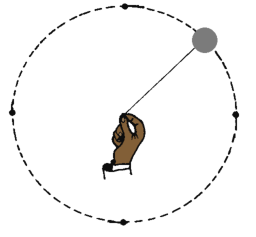
\includegraphics[width=\textwidth]{img/tray_curv.pdf}
  \caption{Una trayectoria curvilínea y circular}
\end{minipage}
\end{figure}

{\color{NavyBlue} \bf En este capítulo nos limitaremos a estudiar los movimientos cuya trayectoria es rectilínea.}

{\bf Para estudiar los movimientos rectilíneos, asociaremos al sistema de referencia un sistema de coordenadas que consiste en una recta que contiene a la trayectoria. En esta recta se indicará el origen $O$ y además se le asignará un sentido. Este sentido estará determinado por el signo positivo para una de las dos semirrectas que quedan determinadas por $O$.}
